%% Q1 q
Match X with Y.\\[2pt]
\begin{tabular}{@{}ll@{}}
\textbf{X} & \textbf{Y}\\
1. Proxemics & a. Use of touch\\
2. Kinesics & b. Use of body language\\
3. Haptics & c. Use of space\\
\end{tabular}

%% Q1
\textbf{Proxemics} is the use of \emph{space} (c), \textbf{Kinesics} the use of \emph{body language} such as gestures, posture and facial expression (b), and \textbf{Haptics} the use of \emph{touch} (a). The match is 1-c, 2-b, 3-a.
\tip{Non-verbal codes: Kinesics (body), Proxemics (space), Haptics (touch), Chronemics (time), Paralanguage (voice qualities), Oculesics (eye contact), Artifacts (dress and objects).}

%% Q2
The use of space and distance in communication is \textbf{Proxemics} (Edward T.~Hall). Hall described four zones: intimate (0--18 in), personal (1.5--4 ft), social (4--12 ft) and public (over 12 ft).
\why{Chronemics = use of time; Paralanguage = tone, pitch, pace and other vocal cues; Haptics = touch.}

%% Q3
\textbf{Connotative meaning} is the associated, emotional or \emph{subjective} meaning that a word carries beyond its dictionary sense. For example, ``home'' connotes warmth and security. \textbf{Denotative} meaning is the literal, dictionary (``real'') meaning.

%% Q4
The receiver \textbf{decodes} the message, interpreting the symbols to extract meaning. The sender encodes, and the channel carries the message.

%% Q5
\textbf{Demophobia} (Greek \emph{demos}, people) is the fear of crowds. It is also called enochlophobia or ochlophobia.
\why{Fear of death = thanatophobia; fear of public speaking = glossophobia; fear of failure = atychiphobia.}

%% Q6
The \textbf{All India Council for Technical Education (AICTE)}, a statutory body under the AICTE Act 1987 (set up as an advisory body in 1945), regulates and ensures the quality of \emph{technical and management} education: engineering, pharmacy, architecture, MBA/PGDM and MCA.
\why{NCERT deals with school curriculum; NCTE with teacher education; NIEPA with educational planning and administration.}

%% Q7
NAAC accreditation is valid for \textbf{5 years}, after which an institution must undergo the next cycle of assessment and accreditation. (NAAC was established in 1994 by UGC and is headquartered in Bengaluru.)

%% Q8
\textbf{National Education Day} is observed on \textbf{11 November}, the birth anniversary of \emph{Maulana Abul Kalam Azad}, India's first Education Minister (1947--58). It has been celebrated since 2008.
\why{14 November is Children's Day (Nehru), 5 September is Teachers' Day (Dr.~S.~Radhakrishnan), and 2 October is Gandhi Jayanti.}

%% Q9
NEP~2020 proposed an \textbf{Academic Bank of Credits (ABC)}, a digital store of the credits earned by students from recognised HEIs. It enables multiple entry and exit, credit transfer and lifelong learning. The UGC ABC Regulations were notified in 2021.

%% Q10
In \textbf{NIRF 2023} (Overall category), \textbf{IIT Madras} was ranked first, as it has been every year since 2019. IISc Bengaluru was 2nd and IIT Delhi 3rd. (IISc tops the \emph{University} category.)

%% Q11 opts
\tikz[baseline=-0.5ex,scale=0.28]{\draw (0,0.45) circle(1); \draw (-0.55,-0.45) circle(1); \draw (0.55,-0.45) circle(1);}
\tikz[baseline=-0.5ex,scale=0.28]{\draw (0,0) circle(1); \draw (1.4,0) circle(1); \draw (2.8,0) circle(1);}
\tikz[baseline=-0.5ex,scale=0.28]{\draw (0,0) circle(1.2); \draw (0,0) circle(0.8); \draw (0,0) circle(0.4);}
\tikz[baseline=-0.5ex,scale=0.28]{\draw (0,0) circle(1.2); \draw (0,0) circle(0.6); \draw (2.2,0) circle(0.7);}

%% Q11
None of the three groups is contained in another, and any two (or all three) can share members. A student may be a tennis fan, a cricket player may be a student, and a student who plays cricket may also be a tennis fan. So the diagram must show \textbf{three mutually overlapping circles} with a common central region, which is option (A).
\begin{center}
\begin{tikzpicture}[scale=0.75,font=\scriptsize]
\draw[fill=brand!10,fill opacity=0.5] (0,0.55) circle(1); \node at (0,1.8) {Tennis fans};
\draw (-0.65,-0.5) circle(1); \node[left] at (-1.65,-0.6) {Cricket players};
\draw (0.65,-0.5) circle(1); \node[right] at (1.65,-0.6) {Students};
\end{tikzpicture}
\end{center}

%% Q12
An \textbf{umpire} presides over and gives decisions in a \textbf{match}; likewise, a \textbf{judge} presides over and decides a \textbf{law suit} (case). The relation is \emph{adjudicator : the event being adjudicated}.
\why{A court is the \emph{place} (the analogue of the stadium), a lawyer is a participant, and a judgement is the decision itself (the analogue of the umpire's ruling).}

%% Q13
A advises B to advertise in newspaper X. This advice assumes that X reaches many people, i.e.\ that it has a wide circulation, so assumption II is implicit. The statement is conditional (``\emph{If} you want to give any advertisement \ldots''), so it does not assume that B actually wants to publicise products. Assumption I is not implicit.
\textbf{Only II is implicit.}

%% Q14
S is P's father and U is S's father, so U is P's paternal \textbf{grandfather}. P is a ``real brother'' of Q, so P is male, a \textbf{grandson}.
\begin{center}
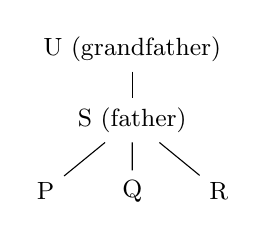
\begin{tikzpicture}[font=\small,level distance=9mm,sibling distance=11mm]
\node{U (grandfather)} child{node{S (father)} child{node{P}} child{node{Q}} child{node{R}}};
\end{tikzpicture}
\end{center}

%% Q15
Three independent patterns:
\begin{itemize}
\item First letters: A, E, I, \textbf{M} (+4 each).
\item Numbers: 7, 12, 19, \textbf{28} (+5, +7, +9).
\item Last letters: T, Q, L, \textbf{E} ($-3$, $-5$, $-7$: T(20)$\rightarrow$Q(17)$\rightarrow$L(12)$\rightarrow$E(5)).
\end{itemize}
The next term is \textbf{M28E}.

%% Q16
All five are web browsers: Microsoft Edge, Google Chrome, Mozilla Firefox, Opera and Apple Safari. The answer is 1, 2, 3, 4 and 5.

%% Q17
All five are video-conferencing tools: Google Meet, Microsoft Teams, Cisco WebEx, Skype and Zoom. The answer is (D).

%% Q18
The first (main entry) page of a website is its \textbf{home page}, usually reached at the site's root URL (e.g.\ \texttt{www.example.com/}). It links to all other sections of the site.

%% Q19
\textbf{Statement I} is true: SWAYAM stands for \emph{Study Webs of Active-Learning for Young Aspiring Minds}.
\textbf{Statement II} is false: not all SWAYAM courses are credit-based. Many are non-credit or certificate courses. Credit transfer (up to 40\% of a programme's credits under the UGC SWAYAM Regulations, 2021) applies only to courses so designated and accepted by the parent university.

%% Q20
The official key accepts both statements, with R explaining A. A router both \emph{receives} data packets (from a network or modem) and \emph{sends} (forwards) them to other devices, so it performs input and output functions at the same time. Its two-way data transfer is the reason it is treated as both an input and an output device.
\tip{Strictly, a router is a \emph{networking} device. In exam questions, devices that both send and receive data (modem, router, touch screen) are usually accepted as ``input--output'' devices.}

%% Q21
Higher education aims at developing independent, critical and self-directed learners. \textbf{Covering every bit of content step by step in class} (spoon-feeding) should be avoided. Guided learning, self-learning, motivation, lectures on difficult content and blended digital learning are all desirable.

%% Q22
A discussion thrives on open-ended, thought-provoking questions. \textbf{Yes/no (closed) questions} have a limited role because they end the exchange with a one-word answer and do not stimulate reasoning or debate.

%% Q23
\textbf{Teaching} involves rational, democratic activities that respect the learner's reasoning: instruction, scientific inquiry, case study and brainstorming. \textbf{Indoctrination} and \textbf{preaching} (sermons) try to implant beliefs without inviting reasoning, so they are not teaching in the true sense.
\why{Options (B), (C) and (D) each contain preaching, sermons or indoctrination.}

%% Q24
The learner variables that largely determine learning outcomes are psychological and academic: \textbf{cognition} (intellectual ability), \textbf{study habits}, \textbf{comprehension} and \textbf{motivation}.
\why{Gender and religion are not determinants of learning outcomes, so any set containing them is wrong.}

%% Q25
Teaching as a profession is characterised by a \textbf{code of conduct (ethics)}, \textbf{professional autonomy} (freedom to work independently) and \textbf{academic freedom} in research and counselling. A \textbf{good income and family life} is a personal benefit, not a defining characteristic that the profession ensures.

%% Q26
SDG~6 (Clean water \& sanitation), SDG~13 (Climate action), SDG~4 (Quality education) and SDG~7 (Affordable \& clean energy) are all goals. \textbf{Deforestation} is a \emph{problem}, not a goal (forests fall under SDG~15, \emph{Life on land}). The answer is 1, 3, 4 and 5.

%% Q27 q
Match the following and choose the correct option given below:\\[2pt]
\begin{tabular}{@{}ll@{}}
\textbf{G20 Presidency year} & \textbf{Nation}\\
I. 2022 & a. Brazil\\
II. 2023 & b. India\\
III. 2024 & c. South Africa\\
IV. 2025 & d. Indonesia\\
\end{tabular}

%% Q27
G20 presidencies: \textbf{2022 Indonesia} (Bali Summit), \textbf{2023 India} (New Delhi Summit; theme \emph{Vasudhaiva Kutumbakam: One Earth, One Family, One Future}), \textbf{2024 Brazil} (Rio de Janeiro), \textbf{2025 South Africa} (Johannesburg). The match is I-d, II-b, III-a, IV-c.

%% Q28
In February 2023 the Geological Survey of India announced inferred lithium resources of about \textbf{5.9 million tonnes} in the \textbf{Salal-Haimana area of Reasi district, Jammu \& Kashmir}, India's first major lithium find. Lithium is vital for EV batteries.

%% Q29
East-coast (Bay of Bengal) cyclones: \textbf{Fani} (May 2019, Odisha) and \textbf{Amphan} (May 2020, West Bengal).
Biparjoy (2023) and Tauktae (2021) struck the \emph{west} coast (Gujarat). The answer is 2 and 4.

%% Q30
An AQI of 257 falls in the \emph{Poor} band (201--300), while an AQI of 65 is \emph{Satisfactory} (51--100). A higher AQI means more air pollution, so City-X is more polluted, and this is exactly what explains the AQI values. Both are true and R explains A.

%% Q31
The scientific method combines \textbf{induction} (observations $\rightarrow$ generalisation or hypothesis) and \textbf{deduction} (hypothesis $\rightarrow$ testable predictions $\rightarrow$ verification). This cycle is called the \textbf{inductive--deductive} method (the ``indo-deductive'' of the option). It is associated with Charles Darwin and John Dewey's reflective thinking.

%% Q32
In \textbf{snowball sampling} each respondent refers further respondents, so the sample ``snowballs''. It suits \textbf{hidden, rare or unknown populations} (drug users, migrant workers, rare-disease patients) for which no sampling frame exists.
\why{It is non-probability, so it does not give a representative sample, and it has nothing to do with a rolling-ball machine.}

%% Q33
Historical research reconstructs the past from documents and relics, and the researcher's interpretation plays a large role. Its findings are therefore \textbf{subjective to a great extent}.
\why{It \emph{is} a scientific inquiry. Sources are validated through external criticism (authenticity) and internal criticism (credibility), so validation is not ``assumptive''. It helps us understand the present and plan for the future.}

%% Q34
A \textbf{discrete variable} takes only separate, countable values (0, 1, 2, \ldots). The \textbf{number of human beings} is counted in whole numbers, so it is discrete.
\why{Height and weight are continuous (they can take any value in a range). IQ is treated as a continuous measure on an interval scale.}

%% Q35
SWAYAM Prabha is a group of 40 \textbf{DTH (Direct-to-Home)} educational TV channels telecasting 24$\times$7 via the GSAT-15 satellite. They are \textbf{free}, cover school, higher and lifelong education, and are not credit-bearing MOOCs.

%% Q36
\begin{center}
\begin{tikzpicture}[scale=0.35,font=\scriptsize,>=Stealth]
\draw[thick,->] (0,0) -- node[left]{4} (0,-4);
\draw[thick,->] (0,-4) -- node[above]{6} (6,-4);
\draw[thick,->] (6,-4) -- node[right]{4} (6,-8);
\draw[dashed,accent,thick] (0,0) -- node[below left]{10} (6,-8);
\fill (0,0) circle(4pt) node[left]{Start};
\end{tikzpicture}
\end{center}
South 4 km, left (east) 6 km, right (south) 4 km. Net: 8 km south and 6 km east.
\[\text{Distance}=\sqrt{8^2+6^2}=\sqrt{100}=\mathbf{10\ km}\]

%% Q37 q
The following diagram shows the number of students who got distinction in the subject out of 500 students.

%% Q37 fig
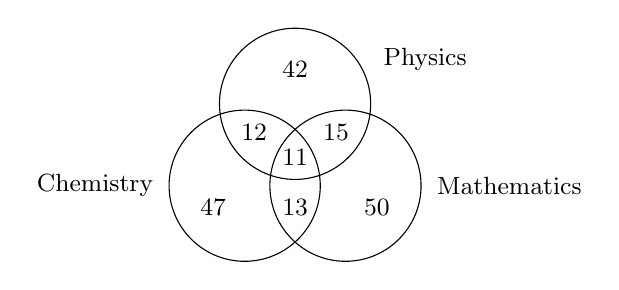
\begin{tikzpicture}[scale=0.8,font=\small]
\draw (0,0.9) circle(1.2); \draw (-0.8,-0.4) circle(1.2); \draw (0.8,-0.4) circle(1.2);
\node at (0,1.45) {42}; \node at (-1.3,-0.75) {47}; \node at (1.3,-0.75) {50};
\node at (-0.65,0.45) {12}; \node at (0.65,0.45) {15}; \node at (0,-0.75) {13}; \node at (0,0.05) {11};
\node[right] at (1.25,1.6) {Physics}; \node[left] at (-2.1,-0.4) {Chemistry}; \node[right] at (2.1,-0.4) {Mathematics};
\end{tikzpicture}

%% Q37 after
What is the percentage of students who got distinction only in two subjects?

%% Q37
``Only two subjects'' means the pairwise overlaps, excluding the centre (11):
\[12\ (\text{P}\cap\text{C})+15\ (\text{P}\cap\text{M})+13\ (\text{C}\cap\text{M})=40\qquad\frac{40}{500}\times100=\mathbf{8\%}\]

%% Q38
When equal \emph{distances} are covered at different speeds, find the total time:
\[t=\frac{25}{25}+\frac{25}{50}+\frac{25}{75}=1+\frac12+\frac13=\frac{11}{6}\text{ h}\qquad \bar v=\frac{75}{11/6}=\frac{450}{11}\approx\mathbf{41\ km/h}\]
(This is the harmonic mean of 25, 50 and 75.)

%% Q39 q
The quarterly sales of a particular mobile in rural and urban areas during year 2022 is as follows:

%% Q39 fig
\begin{tabular}{lcccc}\toprule
\textbf{Area} & \multicolumn{4}{c}{\textbf{Sales in 100 units}}\\\cmidrule(l){2-5}
& Q$_1$ & Q$_2$ & Q$_3$ & Q$_4$\\\midrule
Rural & 30 & 25 & 40 & 35\\ Urban & 40 & 60 & 40 & 70\\\bottomrule
\end{tabular}

%% Q39 after
What is the percentage of sales during Q$_3$?

%% Q39
Total sales $=(30+25+40+35)+(40+60+40+70)=130+210=340$.\\
Q$_3$ sales $=40+40=80$.
\[\frac{80}{340}\times100=\mathbf{23.5\%}\]

%% Q40 q
Given the following data:
\begin{center}
\begin{tabular}{ccccc}
22 & 26 & 18 & 15 & 30\\ 20 & 16 & 22 & 24 & 25\\ 38 & 36 & 28 & 26 & 25\\ 40 & 34 & 36 & 20 & 22\\
\end{tabular}
\end{center}
What is the percentage of observation below average?

%% Q40
Sum of the 20 observations $=111+107+153+152=523$, so the mean $=523/20=26.15$.
Values below 26.15: 22, 26, 18, 15 (row 1); 20, 16, 22, 24, 25 (row 2); 26, 25 (row 3); 20, 22 (row 4), which is 13 values.
\[\frac{13}{20}\times100=65\%\]
65\% is not among the options, which is why the agency \textbf{dropped} the question.

%% Q41 ctx
\textbf{Directions for Q.~41 to 45:} Read the following paragraph and answer the questions given below it.\par\smallskip
You have studied that elemental oxygen is found in the atmosphere in the form of a diatomic molecule (O$_2$). However, in the upper part of the atmosphere, oxygen is present in its triatomic form called ozone (O$_3$). Ozone forms a layer at a height of 15--60 km in the stratosphere. The ozone levels are low over or near the equator and high near the poles.

Ozone is a highly reactive form of molecular oxygen and is poisonous for us. But we are protected from its harmful effects as it is unstable near the surface of the earth. Further, ozone protects the biosphere from the harmful ultraviolet radiations. It filters out the radiations coming to the earth and maintains the temperature of the earth.

Over the last few years, it has been observed that ozone layer is thinning out because of the excessive use of chlorofluorocarbons (CFCs) by human beings. Once considered as miracle compounds, CFCs were being used as propellants in aerosols and as coolants for refrigerators and air conditioners. But now, they are considered harmful compounds as they are stable, do not degrade by any biological process and harm the protective O$_3$ layer by reacting with O$_3$ molecules.

%% Q41
``The ozone levels are \textbf{low over or near the equator} and high near the poles.''

%% Q42
``\ldots oxygen is present in its \textbf{triatomic form} called ozone (O$_3$).''

%% Q43
``Ozone is a \textbf{highly reactive} form of molecular oxygen and is poisonous for us.''

%% Q44
``\ldots ozone protects the biosphere from the harmful \textbf{ultraviolet radiations}.''

%% Q45
``\ldots ozone layer is thinning out because of the \textbf{excessive use of chlorofluorocarbons (CFCs)}.''
\tip{The Montreal Protocol (1987) phases out ozone-depleting substances; 16 September is International Day for the Preservation of the Ozone Layer.}

%% Q46
Let sugar solution $=4x$ and coloured water $=3x$.
\[\frac{4x}{3x+10}=\frac45\Rightarrow20x=12x+40\Rightarrow x=5\]
Initial sugar solution $=4x=\mathbf{20}$ litres.

%% Q47
Profit is shared in the ratio of capital $\times$ time (month-units):
\begin{center}\small
\begin{tabular}{lll}\toprule
Partner & Investment $\times$ months & Total\\\midrule
P & $10{,}000\times5+7{,}000\times7$ & 99{,}000\\
Q & $10{,}000\times5+8{,}000\times7$ & 1{,}06{,}000\\
R & $10{,}000\times5+13{,}000\times7$ & 1{,}41{,}000\\\bottomrule
\end{tabular}
\end{center}
Ratio $=99:106:141$ (sum 346). Shares of Rs.~34{,}600: P $=9{,}900$, Q $=10{,}600$, R $=14{,}100$.

%% Q48
M is on Friday. M is the second ship after J, so J is on \textbf{Wednesday}. K must come before both M and N, and L cannot be on Tuesday. The remaining days (Mon, Tue, Thu) take K, L, N with K before N, e.g.\ K--Mon, N--Tue, L--Thu. Among the options, only ``J is unloaded on Wednesday'' is necessarily true.
\begin{center}\small
\begin{tabular}{ccccc}\toprule Mon & Tue & Wed & Thu & Fri\\\midrule K & N & \textbf{J} & L & \textbf{M}\\\bottomrule\end{tabular}
\end{center}

%% Q49 q
If $+$ means $\times$, $-$ means $+$, $\times$ means $\div$ and $\div$ means $-$, then the value of $6-9+8\times3\div20$ is

%% Q49
Substitute the symbols: $6-9+8\times3\div20$ becomes
\[6+9\times8\div3-20=6+\frac{72}{3}-20=6+24-20=\mathbf{10}\]

%% Q50 q
Three positions of the same dice are given below. Which number will come in place of x?

%% Q50 fig
\die{1}{6}{3}\qquad\die{3}{5}{4}\qquad\die{4}{2}{x}

%% Q50
Die (i): top 1, front 6, right 3. Die (ii): top 3, front 5, right 4. Die (iii): top 4, front 2, right x.
\begin{enumerate}
\item Faces adjacent to 3 are 1, 6 (die i) and 5, 4 (die ii), so \textbf{3 is opposite 2}.
\item Turning die (i) so that 3 comes on top and matching die (ii) gives the opposite pairs \textbf{1--5}, \textbf{6--4}, \textbf{3--2}.
\item In die (iii), 4 is on top (so 6 is at the bottom) and 2 is in front (so 3 is at the back). The two side faces are 1 and 5. Using the orientation fixed by die (i) (with 4 behind and 2 on the left when 1 is on top and 6 in front), bringing 4 to the top and 2 to the front puts \textbf{1 on the right}.
\end{enumerate}
Hence x $=$ \textbf{1}.
